\documentclass[11pt,a4paper]{article}
\usepackage[utf8]{inputenc}
\usepackage[T1]{fontenc}
\usepackage[english]{babel}
\usepackage[top=2.5cm, bottom=2.5cm, left=2.5cm, right=2.5cm]{geometry}
\usepackage{amsmath}
\usepackage{graphicx}
\usepackage{booktabs}
\usepackage{float}      % [H] exact placement
\usepackage{placeins}   % \FloatBarrier
\usepackage{listings}
\usepackage{xcolor}
\usepackage{array}
\usepackage{caption}

% ---------------------------------------------------------------
% Listings style for SQL
% ---------------------------------------------------------------
\lstdefinestyle{sqlstyle}{
    language=SQL,
    basicstyle=\ttfamily\footnotesize,
    keywordstyle=\color{blue!80!black}\bfseries,
    commentstyle=\color{gray}\itshape,
    stringstyle=\color{orange!70!black},
    frame=single,
    rulecolor=\color{black!30},
    breaklines=true,
    numbers=left,
    numberstyle=\tiny\color{gray},
    numbersep=6pt,
    tabsize=2,
    showstringspaces=false,
    captionpos=b
}

\title{Assignment 2: Sustainable Offshore Wind Installation}
\author{Davide Rizzo and Marta Nasso}
\date{April 2026}

\begin{document}

\maketitle

% ---------------------------------------------------------------
\section{Introduction}
% ---------------------------------------------------------------
This report analyses the scheduling problem for a Heavy-Lift Vessel (HLV)
employed in the installation of offshore wind turbines. The objective is to
determine the installation sequence that minimises total fuel consumption by
balancing two contrasting factors:

\begin{itemize}
    \item \textbf{Setup Consumption:} Fuel burned to transit and reconfigure
          the vessel between successive structure types (e.g.\ Monopile to
          Jacket). These costs depend on the ordered pair of consecutive
          structure types and are encoded in a Setup Fuel Matrix.
    \item \textbf{Weather-Window Tardiness Penalty:} The cost incurred by
          missing the designated \emph{Weather Window} for each task. A late
          completion at time $C_j > d_j$ incurs a weighted tardiness charge
          $w_j\,(C_j - d_j)$ plus a fixed remobilisation fee of 100 fuel
          units per late task.
\end{itemize}

The overall cost function to be minimised is therefore:
\begin{equation}
    Z = \underbrace{\text{Setup from Port}}_{\text{first task}} +
        \underbrace{\sum_{i \neq j} S_{ij}\,x_{ij}}_{\text{inter-task setup}}
      + \sum_{j=1}^{n} w_j\,T_j
      + 100\sum_{j=1}^{n} \delta_j
    \label{eq:objective}
\end{equation}
where $T_j = \max(0,\,C_j - d_j)$ is the tardiness of task $j$ and
$\delta_j \in \{0,1\}$ indicates whether task $j$ misses its weather window.

Three solution methodologies are presented: a Mixed-Integer Linear Program
(MILP) formulation solved to global optimality (Approach~A), a Dynamic
Programming (DP) algorithm that exhaustively enumerates all $n!$ permutations
via backward induction (Approach~B), and a Nearest-Neighbour (NN) greedy
heuristic used as a benchmark. Both exact methods are applied to a dataset of
$n = 4$ tasks stored in a relational SQLite database, and their solutions are
compared against the NN heuristic in a sustainability analysis.

% ---------------------------------------------------------------
\section{Task 1: Database Setup}
% ---------------------------------------------------------------
All problem data are persisted in a single SQLite database file
\texttt{offshore\_wind.db} managed through MATLAB's \texttt{sqlite}
interface. The database contains two tables described below.

\subsection{Table Structure}

\paragraph{Deployment\_Schedule.}
Each row represents one installation task, characterised by a structure type,
processing time, logistic weight, and weather-window deadline.

\begin{table}[H]
\centering
\caption{Deployment Schedule — task parameters.}
\label{tab:deployment}
\begin{tabular}{cllrr}
\toprule
\textbf{TaskID} & \textbf{Structure Type} & \textbf{Code} & \textbf{$p_j$ (h)} & \textbf{$d_j$ (h)} \\
\midrule
1 & Monopile & M & 48 & 100 \\
2 & Jacket   & J & 72 & 180 \\
3 & Nacelle  & N & 36 & 120 \\
4 & Monopile & M & 48 & 250 \\
\bottomrule
\end{tabular}
\end{table}

The column \texttt{LogisticsWeight} stores the penalty weight $w_j$: tasks~1
and~4 carry $w = 10$, task~2 carries $w = 8$, and task~3 carries $w = 12$.

\paragraph{Setup\_Fuel\_Matrix.}
Each row stores the fuel cost $S_{\text{from},\text{to}}$ required to
transition between two structure types (or from Port~\texttt{P} to the first
task). The matrix is asymmetric: repositioning from a Jacket to a Monopile is
more expensive than the reverse.

\begin{table}[H]
\centering
\caption{Setup Fuel Matrix — transition costs (fuel units).}
\label{tab:setup}
\begin{tabular}{lrrr}
\toprule
\textbf{From $\backslash$ To} & \textbf{M} & \textbf{J} & \textbf{N} \\
\midrule
P (Port)   & 20 & 30 & 25 \\
M (Monopile) & 5  & 50 & 30 \\
J (Jacket)   & 60 & -- & 40 \\
N (Nacelle)  & 25 & 35 & -- \\
\bottomrule
\end{tabular}
\end{table}

\subsection{SQL Schema and Population}

The database is created by the MATLAB script \texttt{setup\_database.m},
which issues the following SQL statements via the SQLite engine. Using
SQLite requires no external server process: the entire database resides in
a single file and is accessed through MATLAB's built-in \texttt{sqlite}
connector.

\begin{lstlisting}[style=sqlstyle, caption={DDL: table creation.}]
-- Table 1: task scheduling parameters
CREATE TABLE Deployment_Schedule (
  TaskID            INTEGER PRIMARY KEY,
  StructureType     TEXT    NOT NULL,   -- 'M', 'J', or 'N'
  ProcTime          INTEGER NOT NULL,   -- processing time (hours)
  LogisticsWeight   INTEGER NOT NULL,   -- penalty weight w_j
  WeatherWindowEnd  INTEGER NOT NULL    -- deadline d_j (hours)
);

-- Table 2: sequence-dependent setup costs
CREATE TABLE Setup_Fuel_Matrix (
  FromType  TEXT    NOT NULL,
  ToType    TEXT    NOT NULL,
  FuelCost  INTEGER NOT NULL,
  PRIMARY KEY (FromType, ToType)
);
\end{lstlisting}

\begin{lstlisting}[style=sqlstyle, caption={DML: data insertion (Deployment\_Schedule).}]
INSERT INTO Deployment_Schedule
  (TaskID, StructureType, ProcTime, LogisticsWeight, WeatherWindowEnd)
VALUES
  (1, 'M', 48, 10, 100),
  (2, 'J', 72,  8, 180),
  (3, 'N', 36, 12, 120),
  (4, 'M', 48, 10, 250);
\end{lstlisting}

\begin{lstlisting}[style=sqlstyle, caption={DML: data insertion (Setup\_Fuel\_Matrix).}]
INSERT INTO Setup_Fuel_Matrix (FromType, ToType, FuelCost) VALUES
  ('P','M',20), ('P','J',30), ('P','N',25),
  ('M','J',50), ('M','N',30), ('M','M', 5),
  ('J','M',60), ('J','N',40),
  ('N','M',25), ('N','J',35);
\end{lstlisting}

At runtime, both \texttt{solve\_milp.m} and \texttt{solve\_dp.m} open a
read-only connection to \texttt{offshore\_wind.db} and retrieve all
necessary data via \texttt{SELECT} queries before closing the connection.

% ---------------------------------------------------------------
\section{Task 2: Scheduling Optimisation}
% ---------------------------------------------------------------

\subsection{Approach A: Mixed-Integer Linear Programming (MILP)}

\subsubsection{Problem Formulation}

Let $n = 4$ be the number of tasks. Define the following decision variables:
\begin{align*}
    x_{ij} &\in \{0,1\} && \text{1 if task } i \text{ is scheduled immediately before task } j\\
    y_j    &\in \{0,1\} && \text{1 if task } j \text{ is the first task (scheduled from Port)}\\
    s_j    &\geq 0      && \text{start time of task } j \text{ (h)}\\
    C_j    &\geq 0      && \text{completion time of task } j \text{ (h)}\\
    T_j    &\geq 0      && \text{tardiness of task } j \text{ (h)}\\
    \delta_j &\in \{0,1\} && \text{1 if task } j \text{ misses its weather window}
\end{align*}

The \textbf{objective function} minimises total fuel consumption:
\begin{equation}
    \min \quad \sum_{j=1}^{n} \text{port}_j \cdot y_j
             + \sum_{\substack{i,j=1\\i \neq j}}^{n} S_{ij}\,x_{ij}
             + \sum_{j=1}^{n} w_j\,T_j
             + 100\sum_{j=1}^{n} \delta_j
    \label{eq:milp_obj}
\end{equation}
where $\text{port}_j$ is the fuel cost for the transition Port $\to$ task~$j$
and $S_{ij}$ is the setup cost from task~$i$ to task~$j$.

Subject to the following \textbf{constraints}:

\paragraph{C1 — Unique predecessor.} Each task has exactly one predecessor
(either Port or another task):
\begin{equation}
    y_j + \sum_{\substack{i=1\\i \neq j}}^{n} x_{ij} = 1
    \qquad \forall\, j = 1,\ldots,n
    \tag{C1}
\end{equation}

\paragraph{C2 — At most one successor.} Each task has at most one immediate
successor:
\begin{equation}
    \sum_{\substack{j=1\\j \neq i}}^{n} x_{ij} \leq 1
    \qquad \forall\, i = 1,\ldots,n
    \tag{C2}
\end{equation}

\paragraph{C3 — Single first task.} Exactly one task is dispatched first
from Port:
\begin{equation}
    \sum_{j=1}^{n} y_j = 1
    \tag{C3}
\end{equation}

\paragraph{C4 — Completion time.} Completion equals start plus processing:
\begin{equation}
    C_j = s_j + p_j
    \qquad \forall\, j
    \tag{C4}
\end{equation}

\paragraph{C5 — First-task start time.} If $y_j = 1$, the task must start
no earlier than the Port setup time:
\begin{equation}
    s_j \geq \text{port}_j - M\,(1 - y_j)
    \qquad \forall\, j
    \tag{C5}
\end{equation}

\paragraph{C6 — Big-M sequencing.} If $x_{ij} = 1$, task $j$ may not start
before the completion of task $i$ plus the inter-task setup:
\begin{equation}
    s_j \geq C_i + S_{ij} - M\,(1 - x_{ij})
    \qquad \forall\, i \neq j
    \tag{C6}
\end{equation}

\paragraph{C7 — Tardiness lower bound.}
\begin{equation}
    T_j \geq C_j - d_j
    \qquad \forall\, j
    \tag{C7}
\end{equation}

\paragraph{C8 — Late-flag activation.} $\delta_j$ must equal 1 whenever
task $j$ is tardy:
\begin{equation}
    C_j - d_j \leq M\,\delta_j
    \qquad \forall\, j
    \tag{C8}
\end{equation}

A big-M value of $M = 10{,}000$ is employed throughout. The MILP is solved
in MATLAB using \texttt{optimproblem} (Optimization Toolbox).

\subsubsection{Results}

The solver returns the globally optimal sequence:
\begin{equation}
    \text{T3 (N)} \;\to\; \text{T1 (M)} \;\to\; \text{T4 (M)} \;\to\; \text{T2 (J)}
    \label{eq:milp_seq}
\end{equation}

Table~\ref{tab:milp_timeline} details the resulting schedule timeline, and
Table~\ref{tab:milp_breakdown} summarises the cost breakdown.

\begin{table}[H]
\centering
\caption{MILP optimal schedule — timeline and tardiness.}
\label{tab:milp_timeline}
\begin{tabular}{clrrrrrr}
\toprule
\textbf{Slot} & \textbf{Task} & \textbf{Setup (h)} & \textbf{$s_j$ (h)} & \textbf{$C_j$ (h)} & \textbf{$d_j$ (h)} & \textbf{$T_j$ (h)} & \textbf{Late?} \\
\midrule
1 & T3 — Nacelle  & Port$\to$N = 25 & 25  &  61 & 120 &   0 & No  \\
2 & T1 — Monopile & N$\to$M = 25    & 86  & 134 & 100 &  34 & Yes \\
3 & T4 — Monopile & M$\to$M = 5     & 139 & 187 & 250 &   0 & No  \\
4 & T2 — Jacket   & M$\to$J = 50    & 237 & 309 & 180 & 129 & Yes \\
\bottomrule
\end{tabular}
\end{table}

\begin{table}[H]
\centering
\caption{MILP optimal cost breakdown.}
\label{tab:milp_breakdown}
\begin{tabular}{lr}
\toprule
\textbf{Component} & \textbf{Fuel Units} \\
\midrule
Setup from Port (P$\to$N)                & 25    \\
Setup between tasks (N$\to$M + M$\to$M + M$\to$J) & 80    \\
Weighted tardiness ($10\times34 + 8\times129$)     & 1{,}372 \\
Remobilisation ($2 \times 100$)          & 200   \\
\midrule
\textbf{Total}                           & \textbf{1{,}677} \\
\bottomrule
\end{tabular}
\end{table}

\FloatBarrier

\begin{figure}[H]
    \centering
    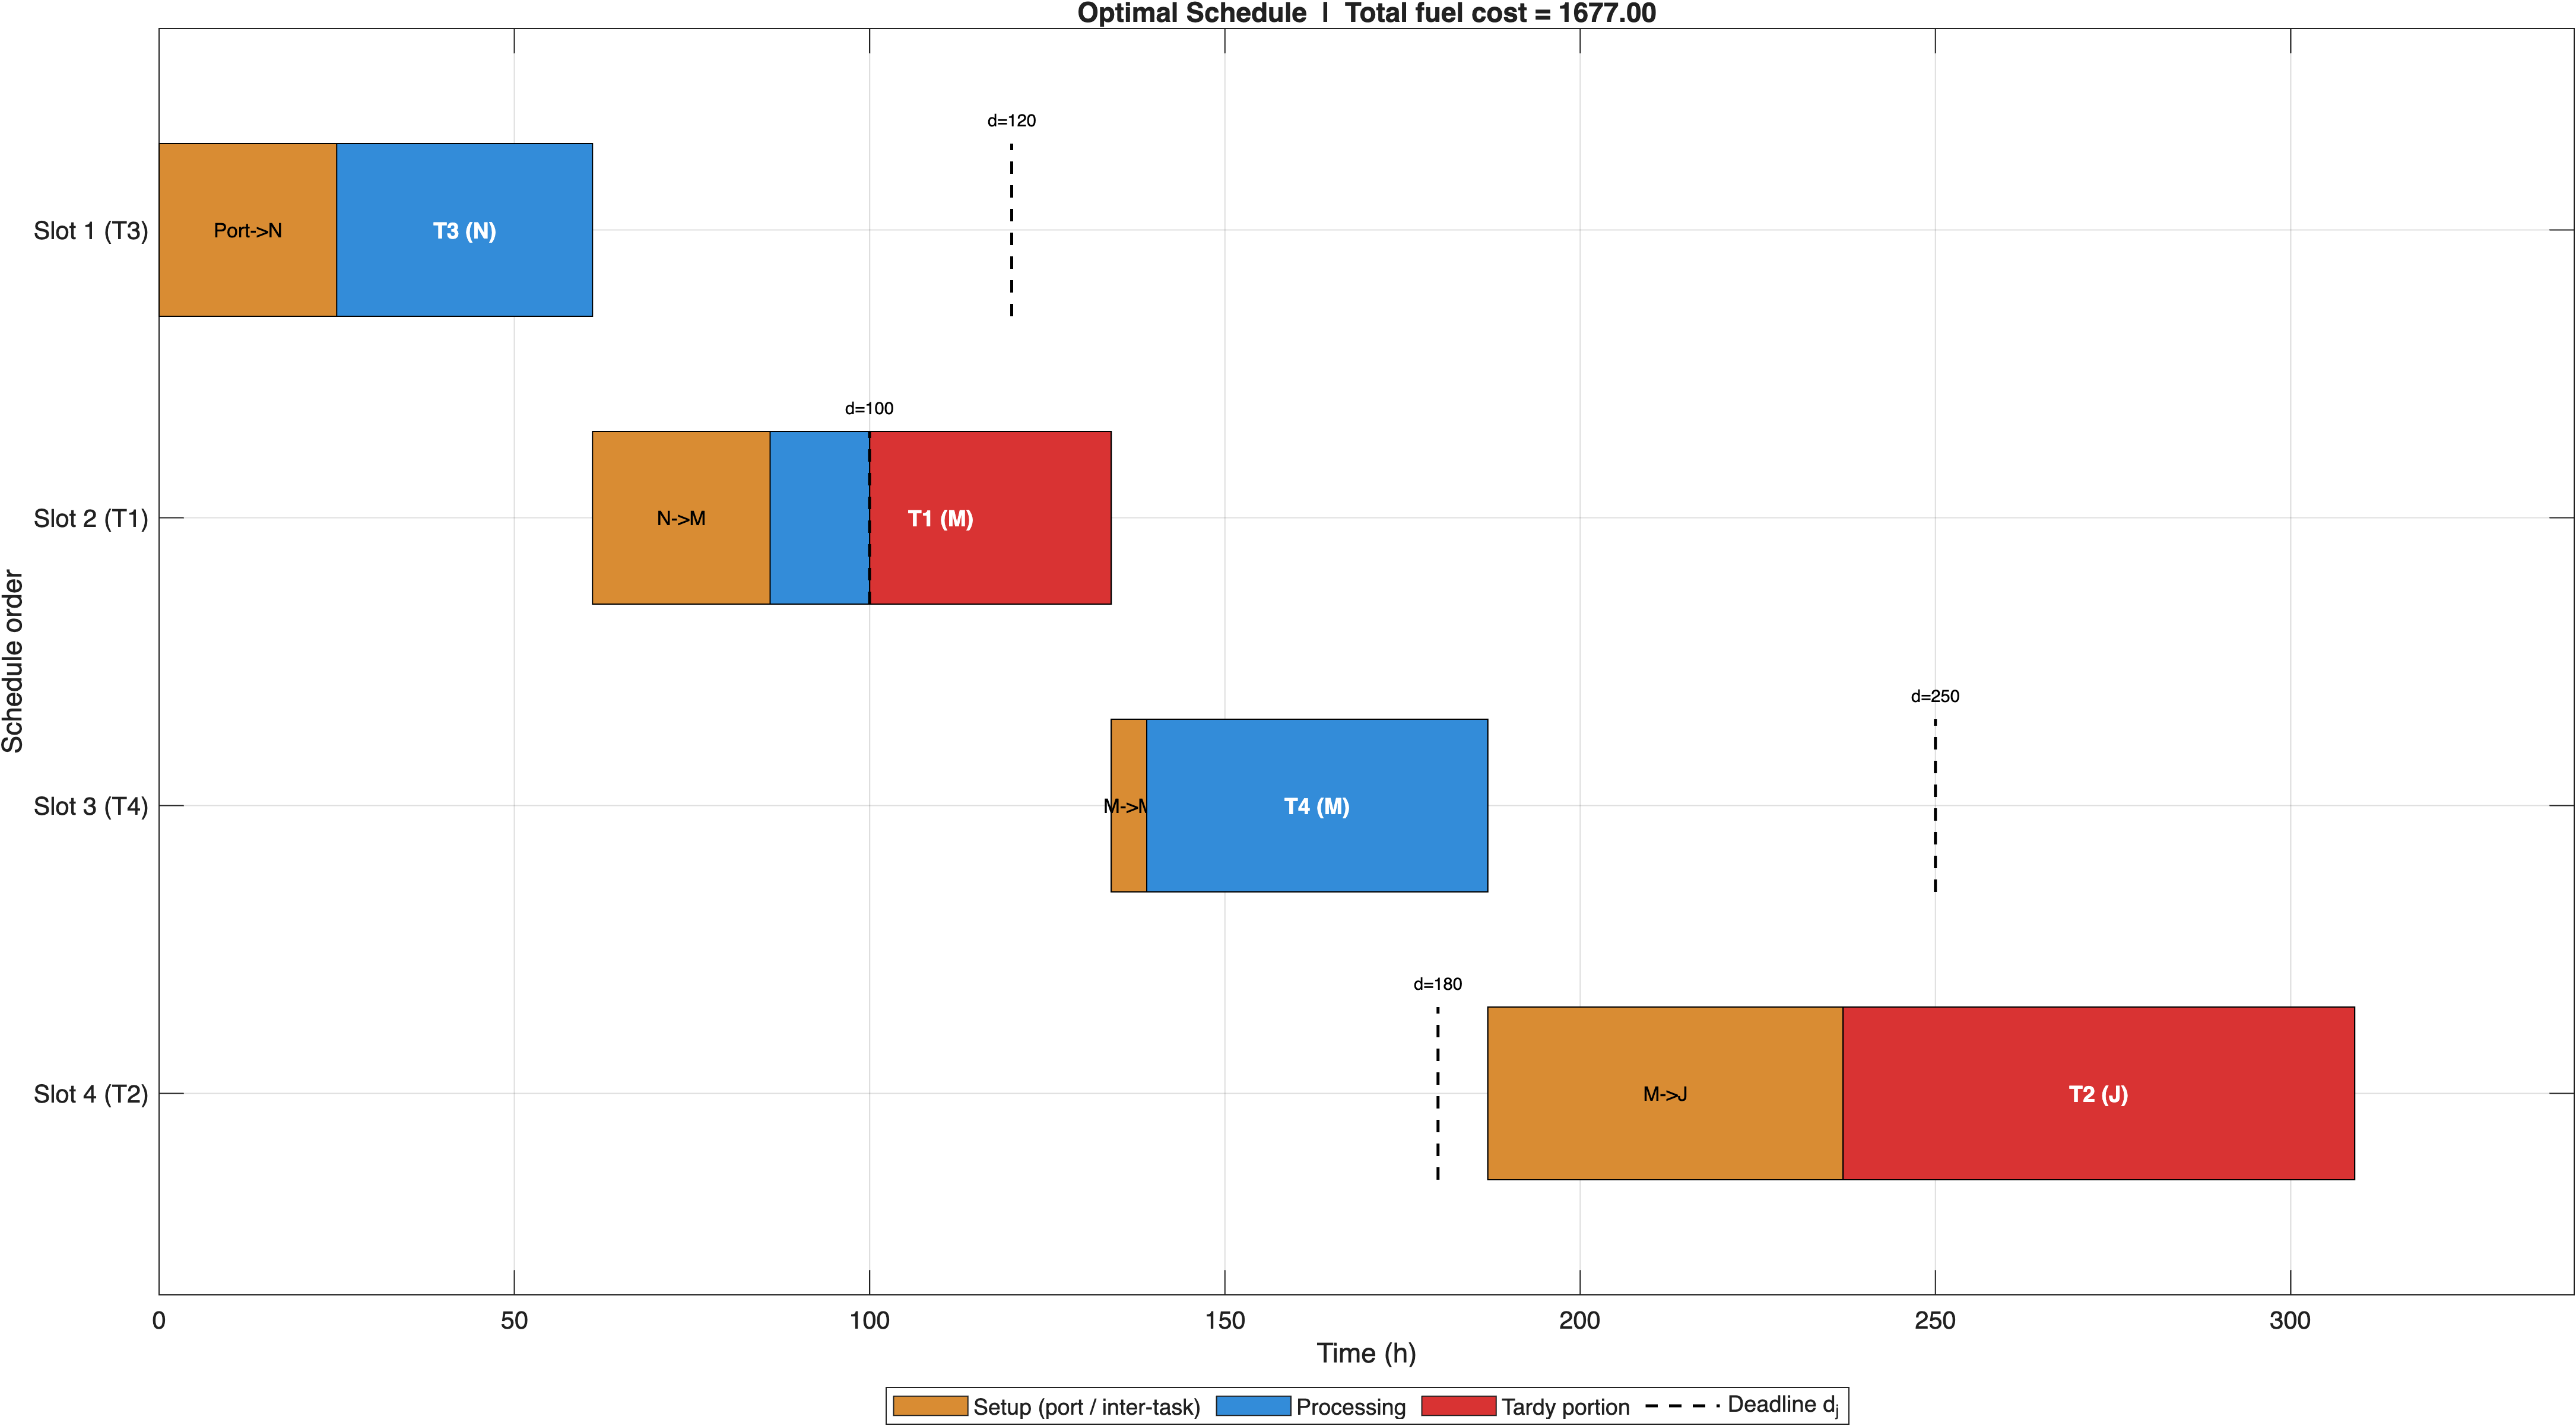
\includegraphics[width=\textwidth]{results/milpGantt.png}
    \caption{Gantt chart of the MILP optimal schedule. Orange bars represent
             setup transitions; blue bars represent on-time processing;
             red bars indicate the tardy portion of a task.
             Dashed vertical lines mark the weather-window deadlines $d_j$.}
    \label{fig:milp_gantt}
\end{figure}

\FloatBarrier

The MILP strategy starts with the Nacelle task (cheapest port setup,
$\text{port}_N = 25$) and then chains the two Monopile tasks back-to-back,
exploiting the very low M$\to$M transition cost of 5 fuel units. The
high-processing-time Jacket task is deferred to the final slot where, despite
its tardiness, the accumulated penalty is lower than any alternative
arrangement.

\subsection{Approach B: Dynamic Programming (DP)}

\subsubsection{Formulation and Algorithm}

Dynamic Programming solves the problem by backward induction over the
\emph{power set} of tasks, following the staged graph structure shown in
Figure~\ref{fig:dp_graph}. The state at stage $k$ is the pair $(S, \ell)$
where $S \subseteq \{1,\ldots,n\}$ with $|S| = k$ is the set of tasks already
completed and $\ell \in S$ is the last task executed. The completion time $t$
is tracked explicitly to evaluate sequence-dependent tardiness penalties.

\medskip
\noindent\textbf{Base case} (stage $n$, all tasks scheduled):
\begin{equation}
    V\!\left(\{1,\ldots,n\},\,\ell,\,t\right) = 0
    \qquad \forall\,\ell,\,t
    \tag{DP-Base}
\end{equation}

\noindent\textbf{Backward recursion} (stage $k = n{-}1,\ldots,1$):
\begin{equation}
    V(S,\ell,t) = \min_{h \notin S}\Bigl\{
        S_{\ell h}
        + w_h\,\max(0,\,t'\! - d_h)
        + 100\cdot\mathbf{1}[t'\! > d_h]
        + V\!\left(S \cup \{h\},\, h,\, t'\right)
    \Bigr\}
    \tag{DP-Rec}
\end{equation}
where $t' = t + S_{\ell h} + p_h$ is the completion time of task $h$.

\noindent\textbf{Initial step} (stage 0, departing from Port):
\begin{equation}
    Z^* = \min_{j=1}^{n}\Bigl\{
        \text{port}_j
        + w_j\,\max(0,\,t_j^{(0)} - d_j)
        + 100\cdot\mathbf{1}[t_j^{(0)} > d_j]
        + V\!\left(\{j\},\,j,\,t_j^{(0)}\right)
    \Bigr\}
    \tag{DP-Init}
\end{equation}
where $t_j^{(0)} = \text{port}_j + p_j$.

The MATLAB implementation (\texttt{solve\_dp.m}) performs a \emph{forward pass}
to enumerate all reachable completion times per state, followed by the backward
DP to compute cost-to-go values, and finally a \emph{forward reconstruction}
to recover the optimal sequence.

The staged graph in Figure~\ref{fig:dp_graph} illustrates all $2^n - 1 = 15$
non-empty subsets across five stages. Each node at stage $k$ corresponds to a
subset of $k$ tasks; edges represent the addition of one task. The highlighted
path traces the optimal solution: $\emptyset \to \{J_3\} \to \{J_1,J_3\} \to
\{J_1,J_3,J_4\} \to \{J_1,J_2,J_3,J_4\}$.

\begin{figure}[H]
    \centering
    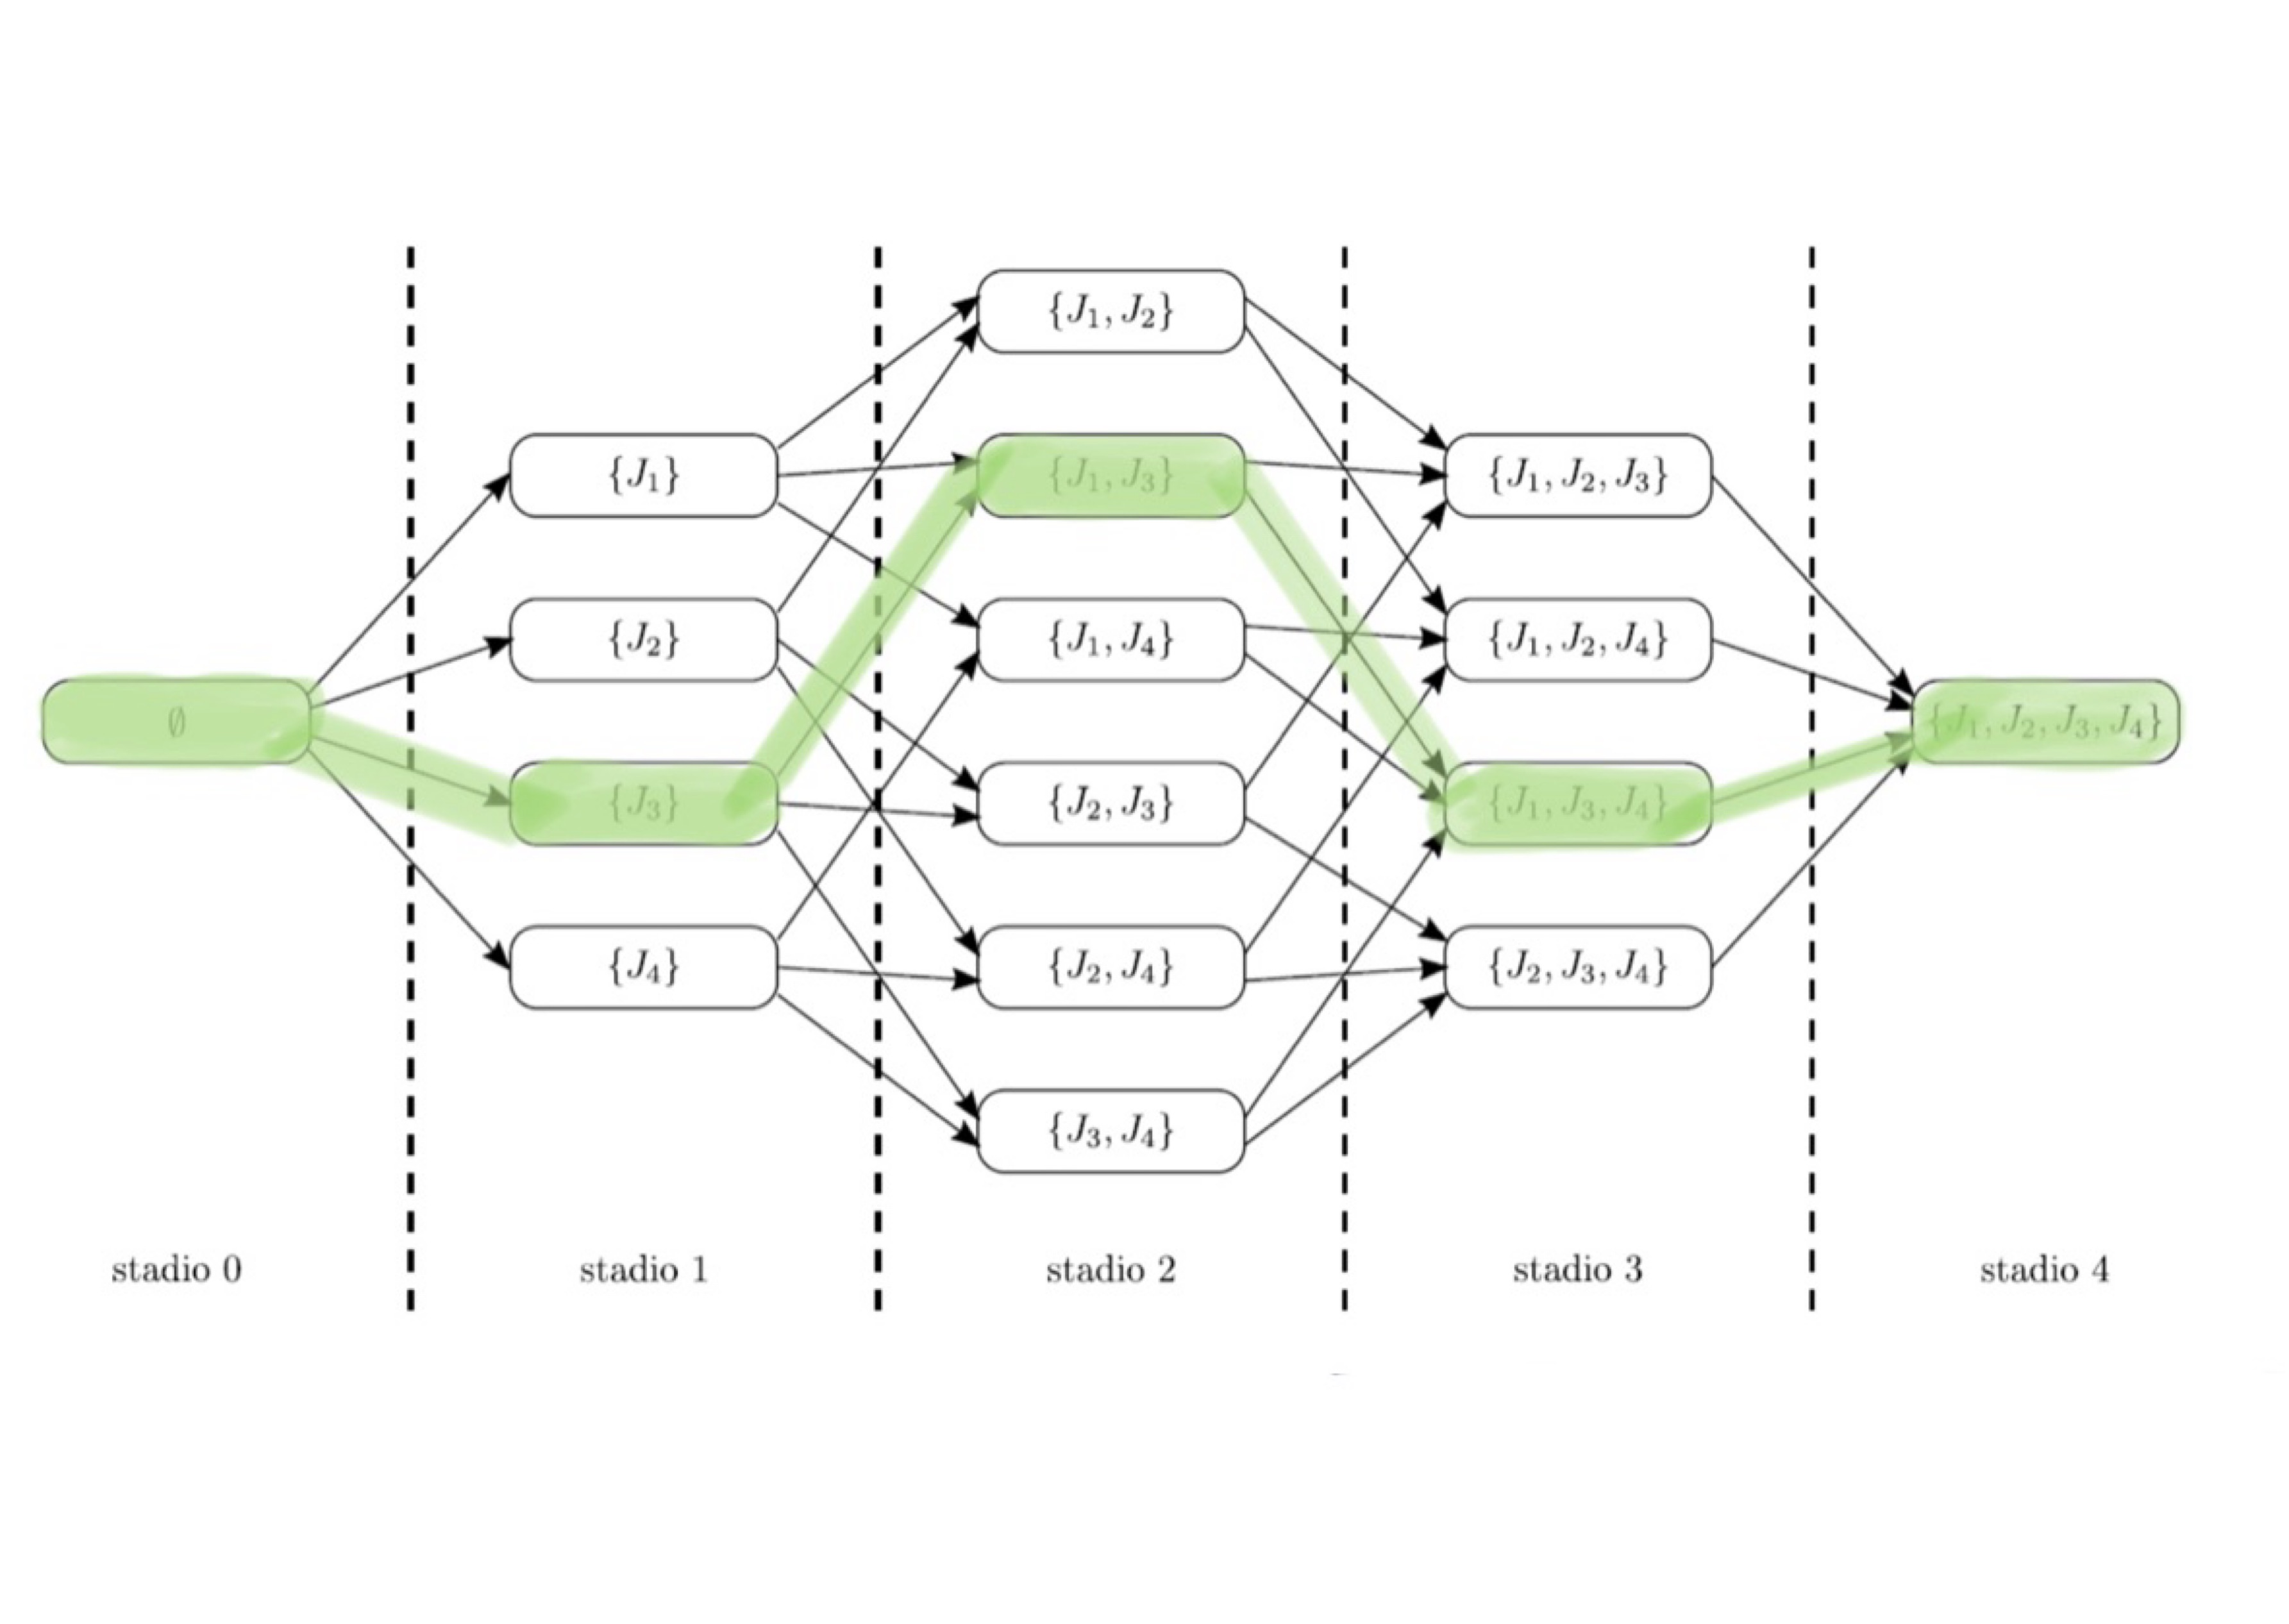
\includegraphics[width=0.85\textwidth]{results/graphDP.jpeg}
    \caption{DP staged graph for $n = 4$ tasks. Each node represents a subset
             of scheduled tasks at the corresponding stage. The highlighted
             (green) path indicates the optimal sequence
             $J_3 \to J_1 \to J_4 \to J_2$.}
    \label{fig:dp_graph}
\end{figure}

\FloatBarrier

\subsubsection{Results}

The DP backward induction yields the identical optimal sequence as the MILP:
\begin{equation}
    \text{T3 (N)} \;\to\; \text{T1 (M)} \;\to\; \text{T4 (M)} \;\to\; \text{T2 (J)}
    \label{eq:dp_seq}
\end{equation}
with a total fuel cost of \textbf{1{,}677 fuel units}, confirming global
optimality. The agreement between the two independent methods validates both
implementations.

\begin{figure}[H]
    \centering
    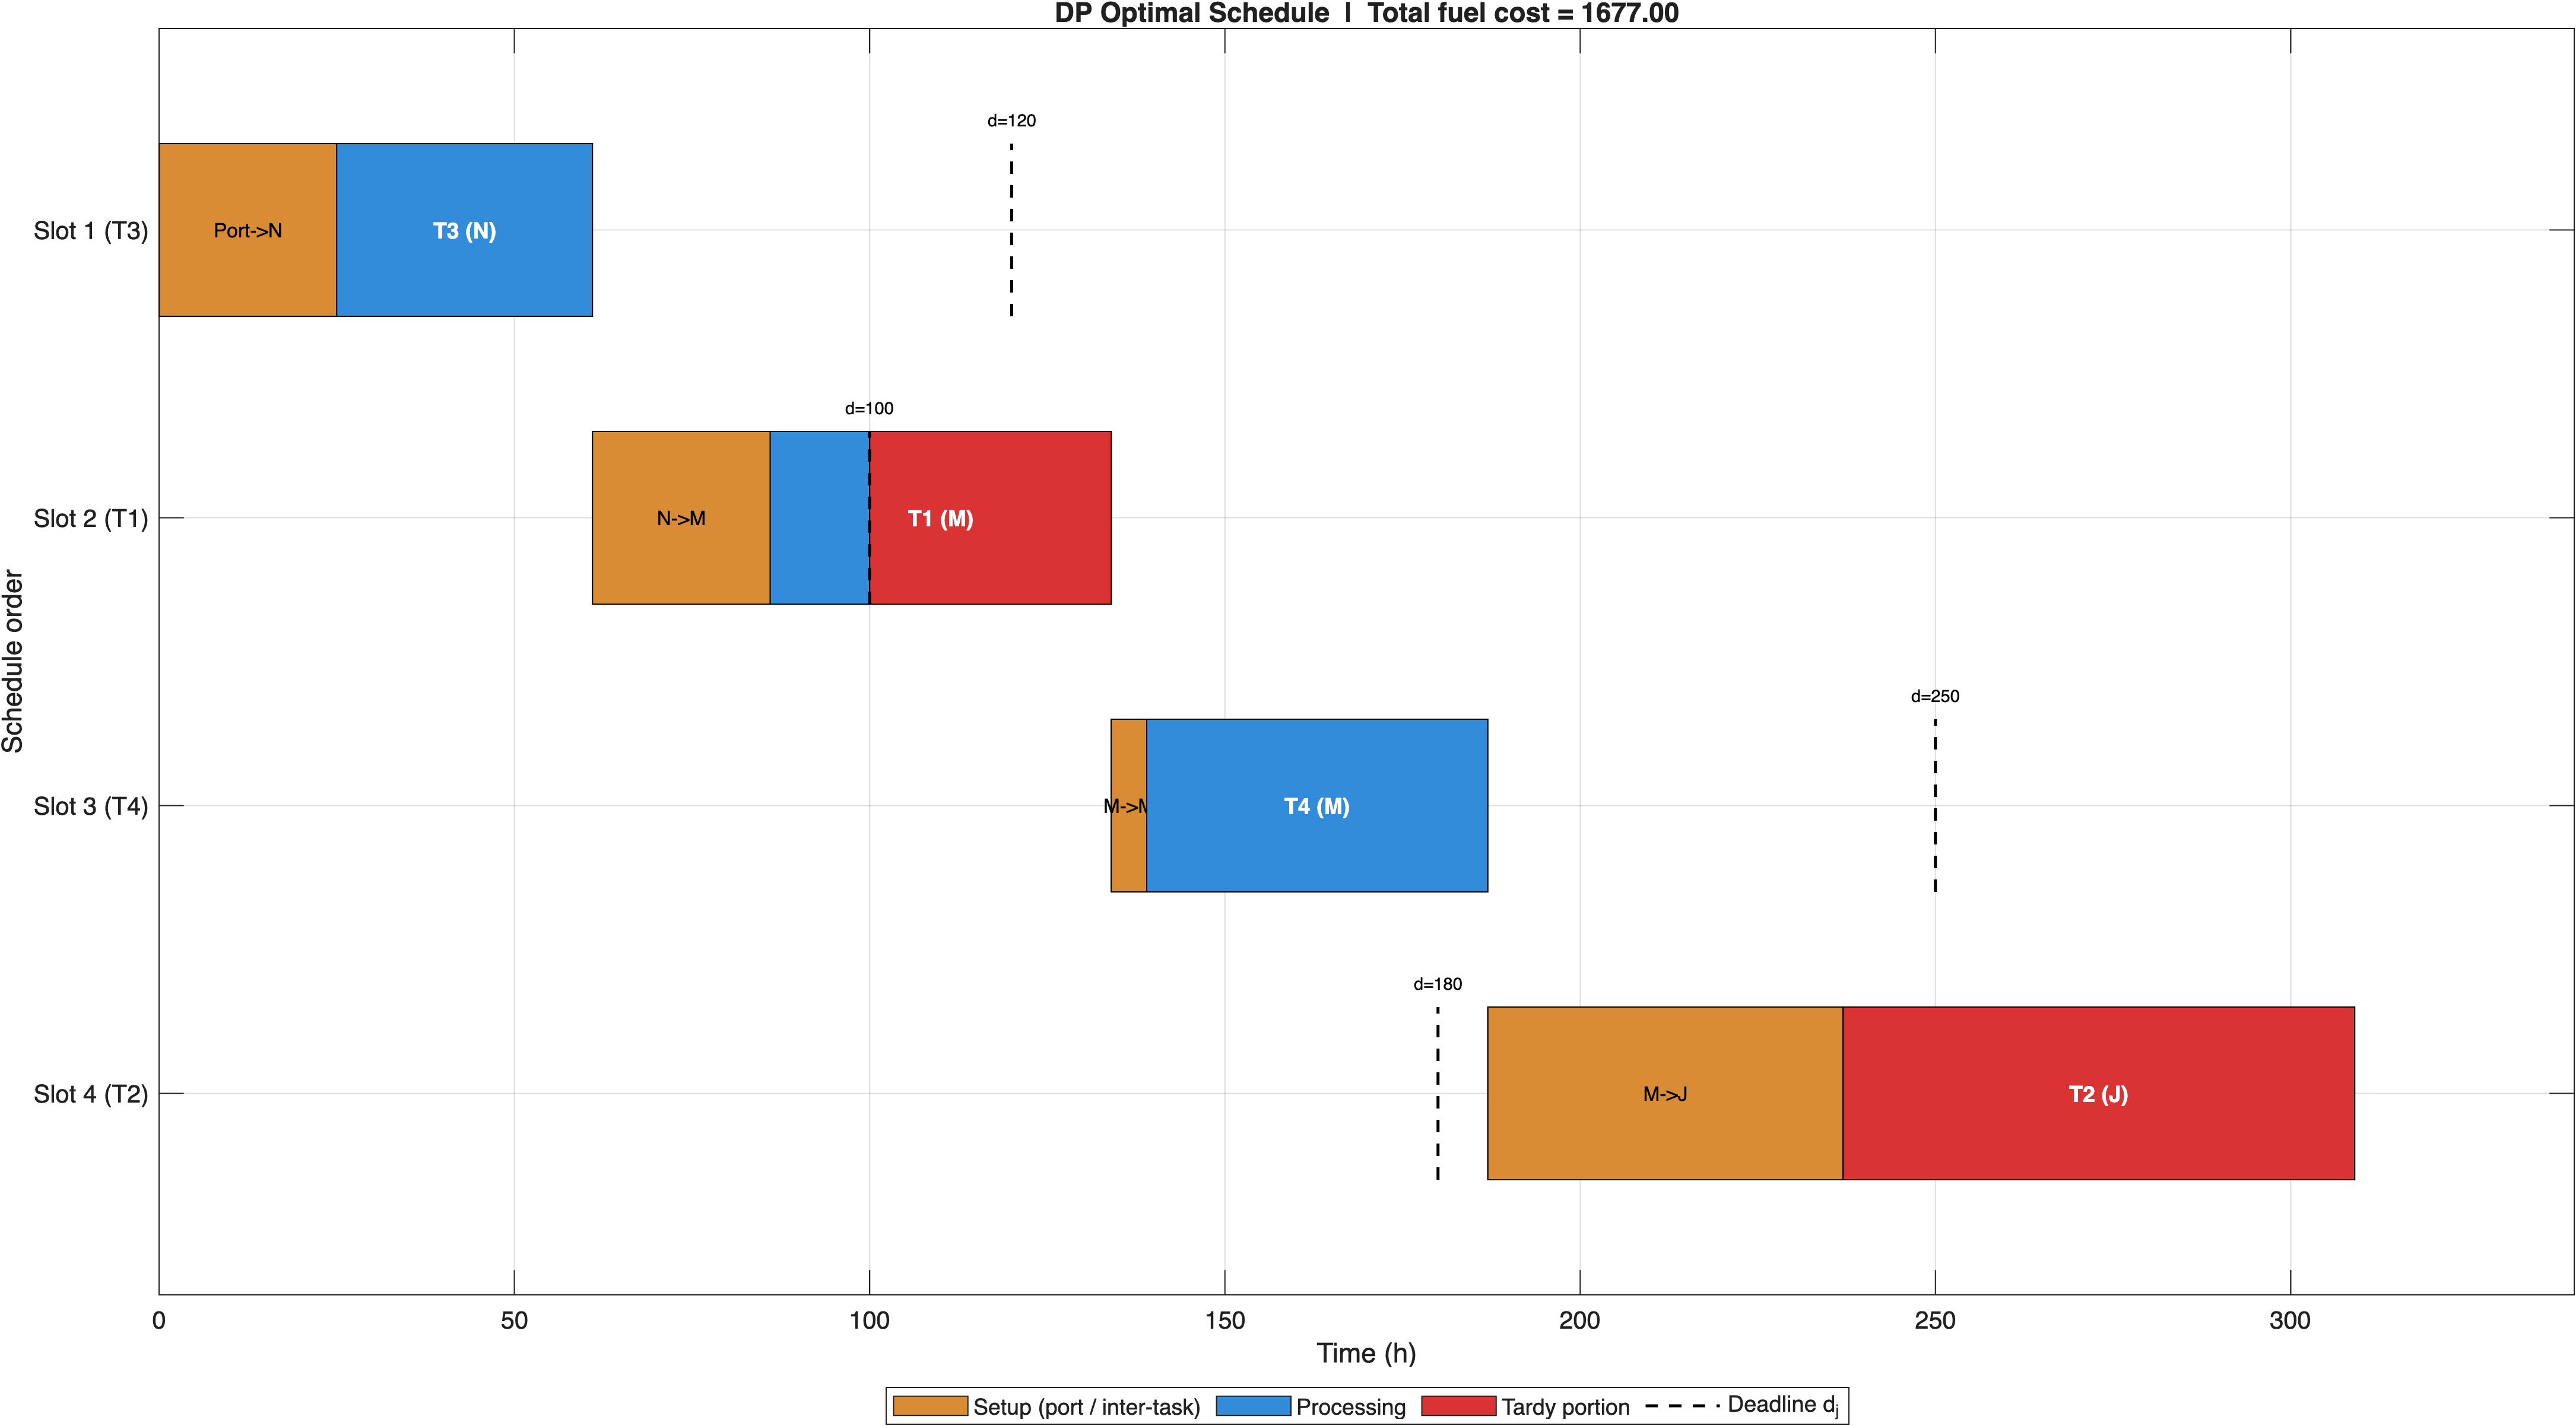
\includegraphics[width=\textwidth]{results/dpGantt.png}
    \caption{Gantt chart of the DP optimal schedule. The layout is identical
             to the MILP result, confirming that both approaches converge to
             the same global optimum.}
    \label{fig:dp_gantt}
\end{figure}

\FloatBarrier

% ---------------------------------------------------------------
\section{Task 3: Sustainability Analysis}
% ---------------------------------------------------------------

\subsection{Nearest-Neighbour Heuristic}

As a baseline, a Nearest-Neighbour (NN) greedy heuristic is applied
(\texttt{nearest\_neighbor.m}). Starting from Port, the algorithm iteratively
selects the unscheduled task with the lowest setup cost from the current
position; ties are broken by smallest \texttt{TaskID}.

\paragraph{NN construction.}
\begin{enumerate}
    \item \textbf{First task:} $\text{port}_M = 20 < \text{port}_N = 25 <
          \text{port}_J = 30$ $\Rightarrow$ select T1 (Monopile; ties with T4
          broken by smallest ID).
    \item \textbf{Second task:} from M, cheapest transition is M$\to$M $= 5$
          $\Rightarrow$ select T4.
    \item \textbf{Third task:} from M, cheapest remaining is M$\to$N $= 30$
          $\Rightarrow$ select T3.
    \item \textbf{Fourth task:} only T2 remains $\Rightarrow$ select T2.
\end{enumerate}

\noindent Resulting NN sequence:
\begin{equation}
    \text{T1 (M)} \;\to\; \text{T4 (M)} \;\to\; \text{T3 (N)} \;\to\; \text{T2 (J)}
    \label{eq:nn_seq}
\end{equation}

Table~\ref{tab:nn_timeline} reports the NN timeline. Compared to the optimal
schedule, the Nacelle task (T3) is delayed to slot~3, causing it to miss its
window ($d_3 = 120$\,h) by 67 hours, whereas the optimal approach completes
T3 in slot~1 with no tardiness.

\begin{table}[H]
\centering
\caption{Nearest-Neighbour schedule — timeline and tardiness.}
\label{tab:nn_timeline}
\begin{tabular}{clrrrrrr}
\toprule
\textbf{Slot} & \textbf{Task} & \textbf{Setup (h)} & \textbf{$s_j$ (h)} & \textbf{$C_j$ (h)} & \textbf{$d_j$ (h)} & \textbf{$T_j$ (h)} & \textbf{Late?} \\
\midrule
1 & T1 — Monopile & Port$\to$M = 20 & 20  &  68 & 100 &   0 & No  \\
2 & T4 — Monopile & M$\to$M = 5     & 73  & 121 & 250 &   0 & No  \\
3 & T3 — Nacelle  & M$\to$N = 30    & 151 & 187 & 120 &  67 & Yes \\
4 & T2 — Jacket   & N$\to$J = 35    & 222 & 294 & 180 & 114 & Yes \\
\bottomrule
\end{tabular}
\end{table}

\subsection{Comparative Cost Breakdown}

Table~\ref{tab:comparison} juxtaposes the cost components of all three
methods. Notably, the NN heuristic achieves a \emph{lower} total setup cost
(90 vs.\ 105 fuel units) because it begins with the cheapest port transition
and chains the two Monopile tasks first. However, this greedy choice
misallocates resources: the Nacelle task, which has the tightest effective
deadline ($d_3 = 120$\,h), is deferred to slot~3, accumulating a large
tardiness penalty.

\begin{table}[H]
\centering
\caption{Cost breakdown comparison across all three methods.}
\label{tab:comparison}
\begin{tabular}{lrrr}
\toprule
\textbf{Component} & \textbf{MILP/DP (optimal)} & \textbf{NN (heuristic)} & \textbf{Difference} \\
\midrule
Setup from Port           &  25     &  20     & $+5$   \\
Setup between tasks       &  80     &  70     & $+10$  \\
\textbf{Total Setup}      & \textbf{105} & \textbf{90} & $\mathbf{+15}$ \\
\midrule
Weighted tardiness        & 1{,}372 & 1{,}716 & $-344$ \\
Remobilisation (late fee) &   200   &   200   &  $0$   \\
\textbf{Total Penalty}    & \textbf{1{,}572} & \textbf{1{,}916} & $\mathbf{-344}$ \\
\midrule
\textbf{Total Cost}       & \textbf{1{,}677} & \textbf{2{,}006} & $\mathbf{-329}$ \\
\bottomrule
\end{tabular}
\end{table}

The optimal methods reduce total cost by \textbf{329 fuel units (16.4\%)}
relative to the NN heuristic. This saving arises entirely from the reduction
in weighted tardiness ($-344$ units), demonstrating that the greedy approach's
lower setup cost is more than offset by its higher penalty costs.

\subsection{Sustainability Interpretation}

Figure~\ref{fig:sustainability} visualises the trade-off between
\emph{Moving Fast} (minimising setup cost by transitioning to the nearest
structure type) and \emph{Waiting} (absorbing higher setup cost to respect
weather windows). In the NN bar, the penalty component dominates strongly,
while the optimal bar shows a significant reduction in the idle DP-mode
penalty at the expense of a slightly larger setup cost.

\begin{figure}[H]
    \centering
    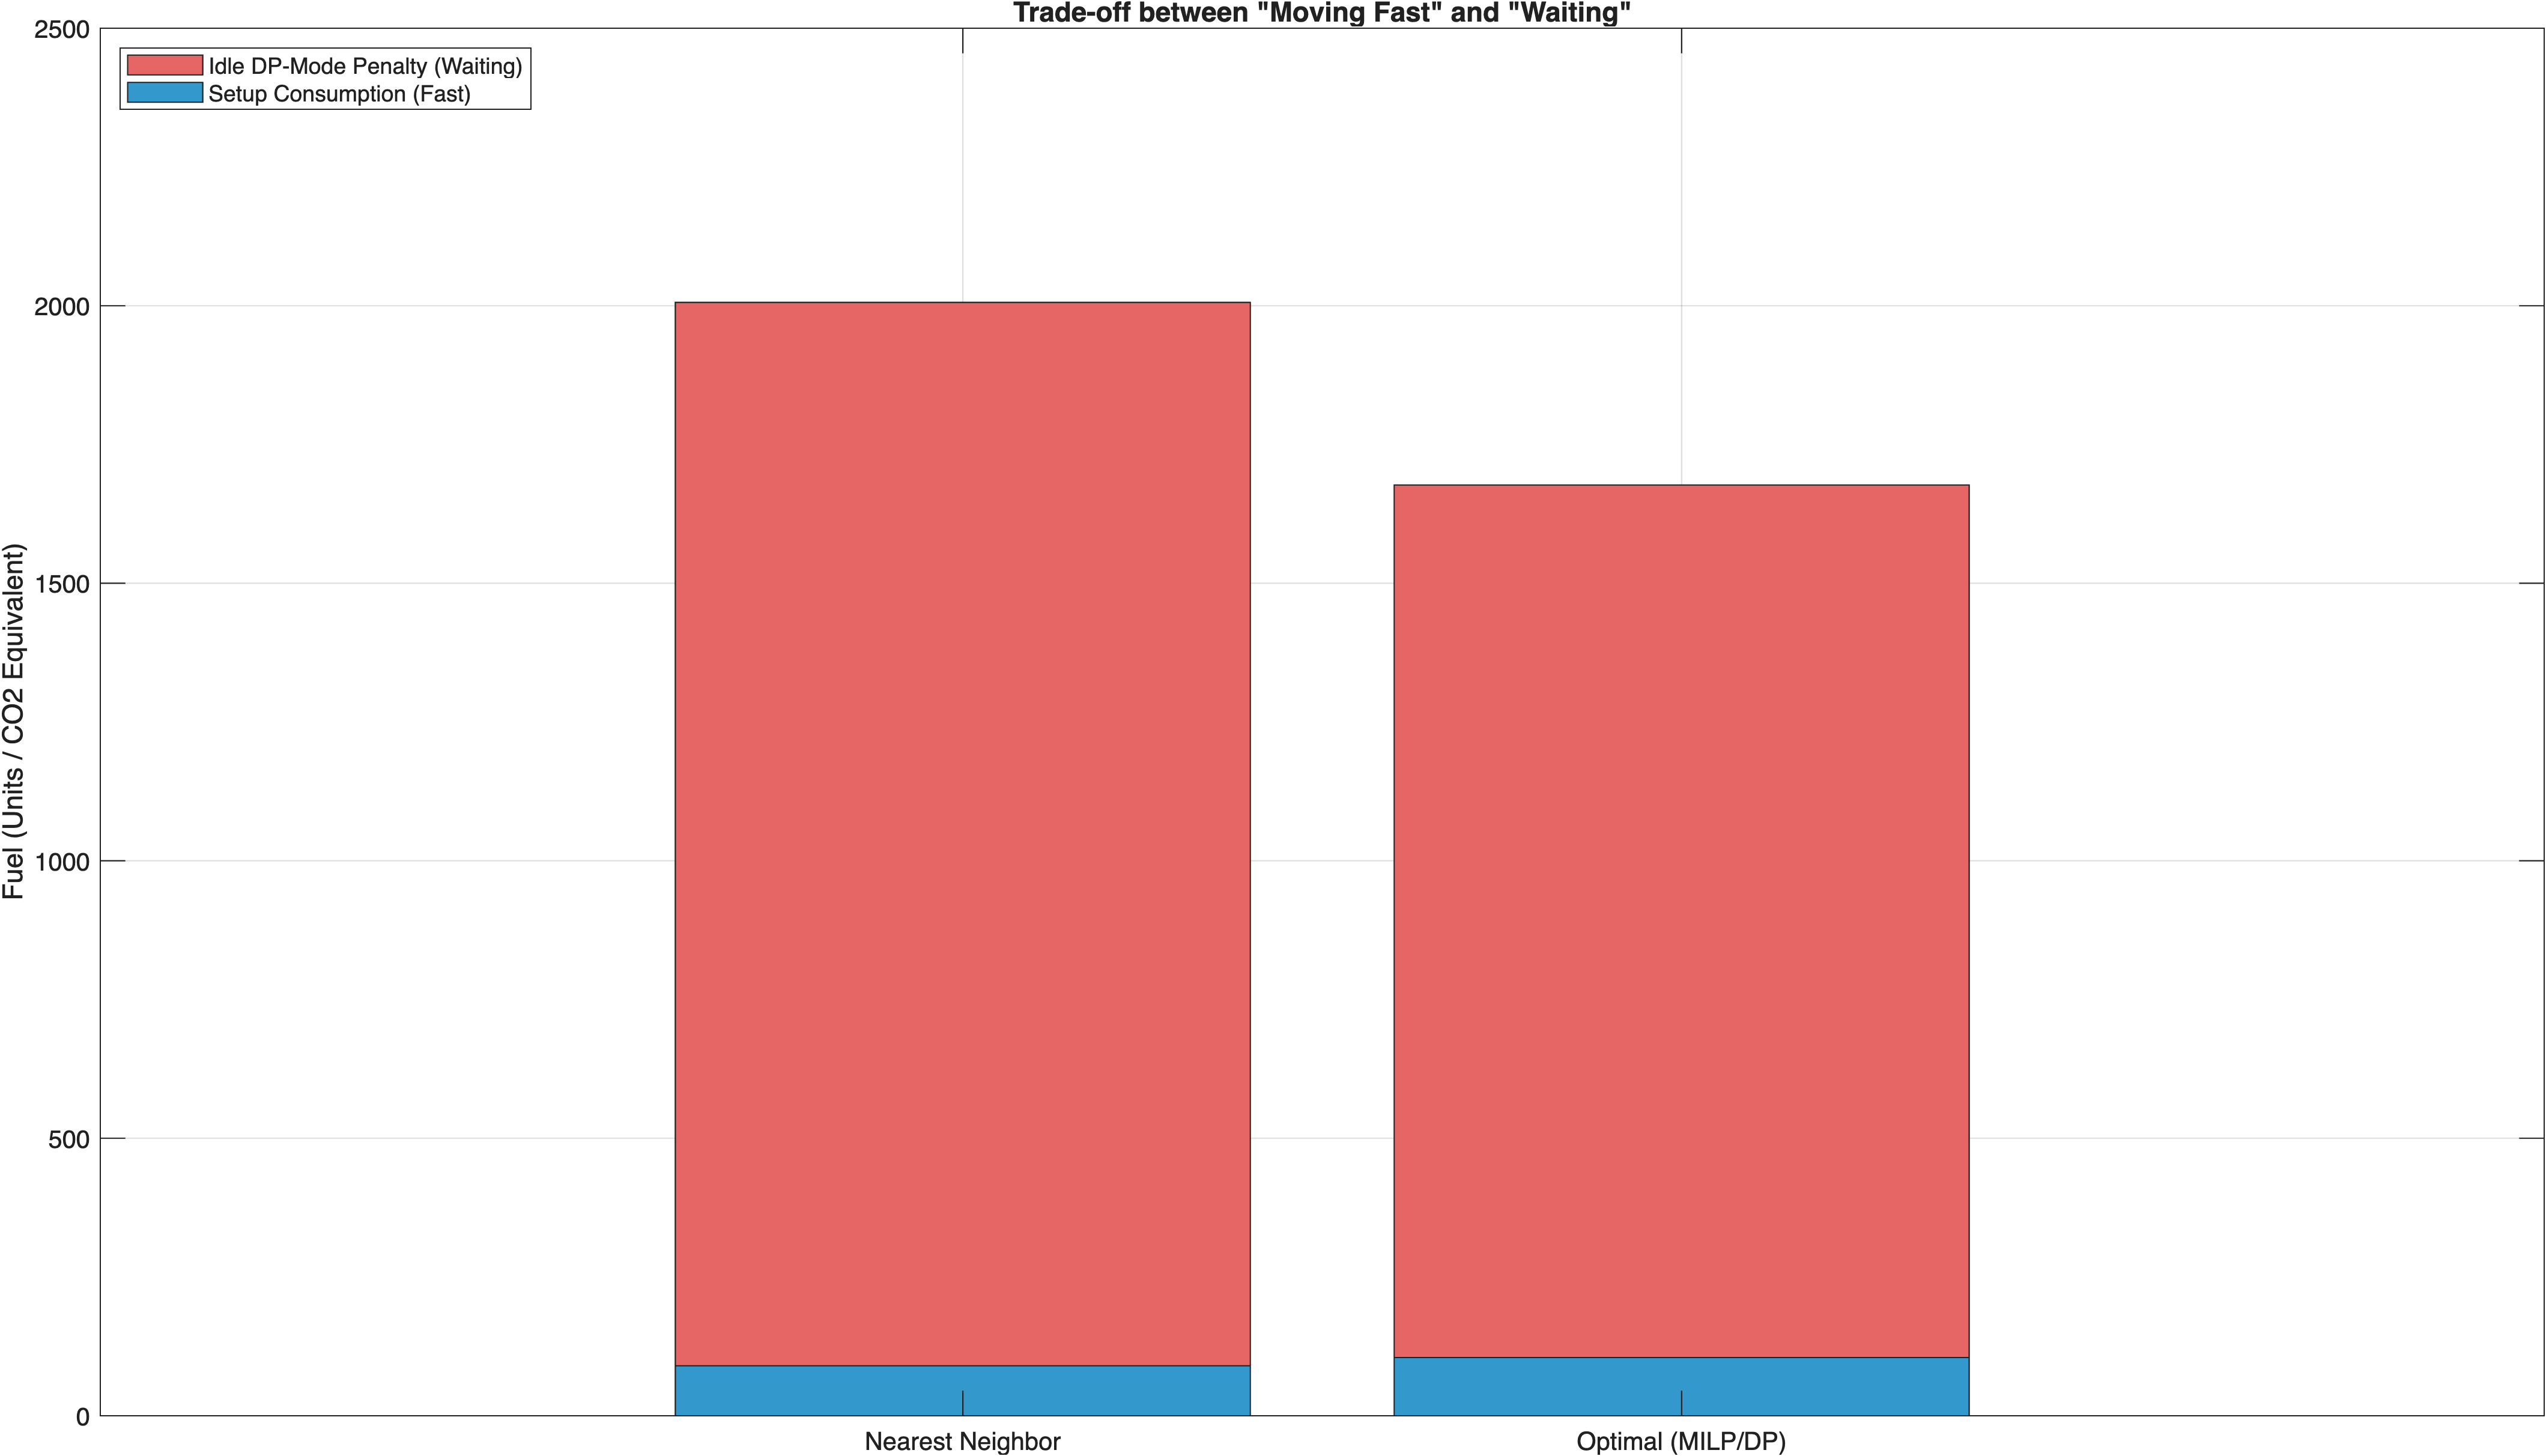
\includegraphics[width=0.85\textwidth]{results/sustainability_plot.png}
    \caption{Stacked bar chart comparing fuel consumption components:
             Setup Consumption (blue, ``Moving Fast'') vs.\ Idle DP-Mode
             Penalty including tardiness and remobilisation (red,
             ``Waiting''). The optimal MILP/DP schedule saves
             329 fuel units (16.4\%) compared to the Nearest-Neighbour
             heuristic.}
    \label{fig:sustainability}
\end{figure}

\FloatBarrier

From a sustainability perspective, each fuel unit can be mapped to a
proportional CO\textsubscript{2}-equivalent emission. The 329-unit saving
represents a material reduction in the vessel's carbon footprint per
installation campaign. The analysis demonstrates that global optimisation
methods — despite their higher computational complexity — provide a
quantifiable environmental benefit beyond mere operational cost savings:
scheduling the Nacelle task first exploits a short processing time and an
early weather window, preventing two separate late-start remobilisation events
and avoiding 344 units of weighted idle fuel burn.

% ---------------------------------------------------------------
\section{Conclusions}
% ---------------------------------------------------------------
This report has addressed the scheduling of $n = 4$ installation tasks for an
offshore wind Heavy-Lift Vessel under sequence-dependent setup costs and
weather-window constraints. Three key findings emerge:

\begin{enumerate}
    \item \textbf{Both exact methods agree.} The MILP and DP formulations
          independently converge to the same optimal sequence
          T3$\to$T1$\to$T4$\to$T2 with a total fuel cost of 1{,}677 units,
          validating the correctness of both implementations.
    \item \textbf{The greedy heuristic is suboptimal.} The Nearest-Neighbour
          approach achieves lower setup cost but incurs 344 additional units
          of tardiness penalty, yielding a 16.4\% higher total cost.
    \item \textbf{Optimisation provides a sustainability benefit.} The 329
          fuel-unit saving directly translates into reduced
          CO\textsubscript{2}-equivalent emissions per campaign, confirming
          that global scheduling optimisation is both economically and
          environmentally preferable.
\end{enumerate}

\end{document}
